\documentclass[a4paper,9pt]{report}

/stock/16_git_repo/library/library.tex

\begin{document}
% {{{ Page de garde
%../../../../00_resources/page_garde.tex
% }}}

% {{{ Première partie : sans titre pour l'instant
% TODO Split en plusieurs fichiers

\chapter{Pr\'{e}sentation des problèmes}

% TODO Introduction avec définition général des problèmes d'ordonnancement et présentation des
% différentes possibilités + Introduction du modèle
% TODO Présentation de l'interval Scheduling et du problème de réservation de l'hotel
% TODO Présentation du modèle de notation à trois champs

\section{Introduction}
\subsection{Motivations}

Faire une présentation du problème de réservations dans un hôtel, parler flexibilité

\subsection{L'ordonnancement}

Choses à faire :
\begin{itemize}
    \item présentation du domaine
    \item définition d'un ordonnancement
    \item introduction à la notation à trois champs
\end{itemize}

\section{Définitions}

% {{{ DEF : Tache
\begin{ndf}[Tâche]
    Une tâche est une entité élémentaire indivisible dont la réalisation nécessite une certaine
    quantité de ressources, dans notre cas un certain temps de calcul d'une machine. Considérons une
    tâche $j$, elle est caractérisée par une date de début $\st{j}$ et une date de fin $\ct{j}$ et donc
    représentable par un intervalle de la forme $[\st{j}, \ct{j}]$ avec $\st{j} < \ct{j}$. La durée d'exécution
    de la tâche est notée $\pt{j}$ et est définie par : $\pt{j} = \ct{j} - \st{j}$.

    L'ensemble des tâches considérées est noté $\mathcal{T}$.
\end{ndf}
% }}}

\begin{nrmq}
    Par la suite nous nous restreindrons à des tâches dont les dates de début et de fin sont à
    valeurs entières et positives.
\end{nrmq}

% {{{ DEF : Réservation
\begin{ndf}[Réservation]
    Étant donnée une machine $m_i$, une réservation sur $m_i$ est une plage d'activité ou
    d'inactivité de la machine pendant laquelle les ressources de calcul de cette dernière sont
    indisponibles. Une réservation $l$ est caractérisée par une date de début $\sres{l}$ et une date de fin
    $\cres{l}$ et est relatif à une machine donnée. Elle est donc représentable par un couple composé
    d'une machine $m_i$ et d'un intervalle de la forme $[\sres{l}, \cres{l}]$ avec $\sres{l} < \cres{l}$.
    La durée d'une réservation $\pres{l}$ est définie par :  $\pres{l} = \cres{l} - \sres{l}$.

    L'ensemble des réservations considérées est noté $\mathcal{R}$.
\end{ndf}
% }}}

%{{{ RMQ : Événements
\begin{nrmq}
    Nous appellerons \emph{événement} tout entité étant soit une tâche soit une réservation.
    L'ensemble des événement sera noté $\mathcal{E} = \mathcal{T} \cup \mathcal{R}$.
\end{nrmq}
% }}}

% {{{ DEF : Trou
\begin{ndf}[Trou]
    Étant donnés un ensemble de machine $\mathcal{M} = \{m_1, m_2, \dots, m_k\}$, un ensemble de
    tâches $\mathcal{T}$ et un ordonnancement $\mathcal{O}$ de ces tâches sur $\mathcal{M}$, un trou
    dans l'ordonnancement $\mathcal{O}$ est une plage d'inactivité non nulle de la machine, pendant
    laquelle les ressources de calcul de cette dernière sont disponibles et peuvent être utilisées à
    la réalisation d'une tâche. Un trou $\eta$ est caractérisé par une date de début $\sho{\eta}$ et
    une date de fin $\cho{\eta}$ et est relatif à un ordonnancement et à une machine. Il est donc
    représentable par un triplet composé d'un intervalle de la forme $[\sho{\eta}, \cho{\eta}]$ avec
    $\sho{\eta} < \cho{\eta}$, d'un ordonnancement et d'une machine. La durée d'un trou est donnée
    par $\pho{\eta} = \cho{\eta} - \sho{\eta}$.
\end{ndf}
% }}}

% {{{ REMARQUE : PRESENTATION DES CAS
\begin{nrmq}
    Nous illustrons ces notions à la figure~\ref{prescas}, les rectangles gris
    représentent différentes tâches, les rectangles noirs sont les réservations alors que les plages
    libres représentent les différents trous possibles.
\end{nrmq}
% }}}

Nous aurons besoin de définir la notion de graphe d'intervalles propre utilisée en
section~\ref{scomplexite}.

% {{{ DEF : GRAPHE D'INTERVALLE
\begin{ndf}[Graphe d'intervalles]
    Étant donné un ensemble d'intervalles $\mathcal{I} = \{b_1, \dots, b_n\}$ tels que $b_i = [\sint{i},
    \cint{i}]$, le graphe d'intervalles défini par cet ensemble est un graphe non orienté construit de la
    manière suivante :
    \begin{enumerate}
        \item à chaque intervalle $b_i \in \mathcal{I}$ on associe un sommet $v_i$.
        \item étant donnés deux sommets $v_i,\ v_j \in V$, $[v_iv_j) \in E$ si et seulement si 
            $\sint{i} \leq \sint{j} < \cint{i}$ ou $\sint{j} \leq \sint{i} < \cint{j}$. Il s'agit
            de la manière formelle de dire qu'une arête existe entre deux sommets $v_i$ et $v_j$ si
            et seulement s $i$ et $j$ se chevauchent.
    \end{enumerate}

    Un graphe d'intervalles est dit propre si et seulement si, étant donnés deux intervalles $b_i$
    et $b_j$ : $\sint{i} \leq \sint{j} < \cint{i} \Rightarrow \cint{j} > \cint{i}$

    Autrement dit, il n'existe aucun intervalle inclus dans un autre.
\end{ndf}
% }}}

\section{Les problèmes considérés}

\subsection{Définition}

À l'aide des notions développées précédemment, nous définissons le problème suivant :

% {{{ PROBLEME : Flexible Interval Scheduling
\dfopt{\fisched}
{Un ensemble $\mathcal{M} = \{m_1, \dots, m_k\}$ de $k$ machines, un ensemble $\mathcal{T} = \{j_1,
    j_2, \dots j_n\}$ de tâches avec $j_i$ représentant l'intervalle $[\st{j_i}, \ct{j_i}]$, un
ensemble $\mathcal{R}$ de réservations $l = (m_i, [\sres{l}, \cres{l}])$.} 
{Un ordonnancement $\mathcal{O}$ des tâches sur les $k$ machines maximisant le trou
minimum.}
% }}}

et son problème de décision associé :

% {{{ PROBLEME : Flexible Interval Scheduling Decision
\dfdec{\fischedpi}
{Un ensemble de $k$ machines, un ensemble $\mathcal{T} = \{j_1, j_2, \dots, j_n\}$ de tâches avec
    $j_i$ représentant l'intervalle $[\st{j_i}, \ct{j_i}]$, un ensemble $\mathcal{R}$ de
réservations $l = (m_i, [\sres{l}, \cres{l}])$, un entier $z$.}
{Existe-t-il un ordonnancement $\mathcal{O}$ des tâches sur les $k$ machines tel que la taille du
trou minimum soit au moins égale à $z$?}
% }}}

\subsection{Formalisation}
% {{{ REMARQUE : Formalisation
    Si l'on considère la fonction d'affectation de tâches sur les machines\footnote{Par la suite
    nous noterons cette fonction $f$ en lieu et place de $f_{\mathcal{O}}$.}: \[
        f_{\mathcal{O}} : \left \lbrace \begin{array}{rcl}
            \mathcal{T} \cup \mathcal{R} & \longrightarrow & \mathcal{M} \\
            j & \mapsto & f_{\mathcal{O}}(j) \\
        \end{array}
        \right .
    \]
    qui, étant donné un ordonnancement $\mathcal{O}$, associe à une tâche ou une réservation $j$, la
    machine $m_i$ sur laquelle s'exécute cette tâche pour l'ordonnancement donné\footnote{Dans le
    cas d'une réservation, le résultat de la fonction est indépendant de l'ordonnancement
    considéré.}, on peut alors définir de manière plus formelle : \begin{bitemize}
        \item l'ensemble des tâches : \hfill $ \mathcal{T} = \{[\st{j}, \ct{j}]   \colon  
            \ct{j} - \st{j} = \pt{j} \} $
        \item l'ensemble des réservations : \hfill $\mathcal{R} = \{l = (m_p, [\sres{l}, \cres{l}])  
            \colon   \cres{l} - \sres{l} = \pres{l},\ f(l) = m_p\}$
        \item la fonction objectif étudiée : \hfill $H_{\min} = \min \{ \cgen{i} - \sgen{i'} > 0  
            \colon   i,i' \in \mathcal{T} \cup \mathcal{R},\ f(i) = f(i')\}$
    \end{bitemize}

    On peut finalement définir la notationà trois champs de ce problème, à savoir : 
    \begin{center}
        $P \arrowvert \mbox{Intervalle},\ \mathcal{T},\ \mathcal{R} \arrowvert H_{\min}$
    \end{center}
    
% }}}

% {{{ REMARQUE : Conventions
\subsection{Conventions}
    Quelques conventions sur les problèmes étudiés : \begin{enumerate}
        \item la date de début d'un ordonnancement est fixée à $- \infty$ de façon à
            ce que les trous initiaux aient une taille infinie. Ainsi sur la figure~\ref{prescas},
            on a : $\pho{h_4} = \pho{h_7} = \infty$.
        \item la date de fin d'un ordonnancement est fixée, quant à elle, à
            $+\infty$ de manière à ce que les trous finaux aient eux aussi une taille infinie. On a
            alors : $\pho{h_5} = \pho{h_6} = \infty$.
        \item le temps $t_0$ est défini comme suit : \[
                t_0 = \min\{\min\{\st{j} : j \in \mathcal{T}\}, \min\{\sres{l} : l \in \mathcal{R}\}\}
            \]
            $t_0$ représente le point $0$ de l'échelle de temps relative utilisée pour les
            intervalles.

            Considérons l'ensemble d'intervalles $\mathcal{I} = \{[3,9], [5,10], [9,11]\}$, dans ce
            cas $t_0 = 3$ et nous utiliserons l'ensemble d'intervalles $\mathcal{I}' = \{[0,6],
            [2,7], [6,8]\}$.
    \end{enumerate}

    Par conséquent, pour la fonction objectif étudiée, nous ne
    nous intéressons que aux trous délimités à gauche et à droite par une tâche ou un réservation.
% }}}

% {{{ FIGURE : Différents cas de figure
\begin{figure}
    \begin{center}
        \begin{ordo}[10]{3}{1}{9}
            \newtask{2}{1}{1}{$t_1$}
            \newtask{1}{1}{7}{$t_2$}
            \newhole{4}{1}{3}{$h_1$}Optimisation

            \newlabeledresa{2}{2}{0}{$l_1$}
            \newtask{3}{2}{4}{$t_3$}
            \newhole{2}{2}{2}{$h_2$}

            \newlabeledresa{3}{3}{2}{$l_2$}
            \newlabeledresa{2}{3}{7}{$l_3$}
            \newhole{2}{3}{5}{$h_3$}

            \newbeghole{1}{1}{$h_4$}
            \newbeghole{2}{3}{$h_7$}

            \newendhole{1}{1}{8}{$h_5$}
            \newendhole{2}{2}{7}{$h_6$}
        \end{ordo}
    \end{center}
    \caption{Illustration des différents cas de figures}
    \label{prescas}
\end{figure}
% }}}

% {{{ FIGURE : Exemple ordonnancement
\begin{figure}
    \begin{center}
        \begin{ordo}[10]{3}{1}{10}
            \newlabeledresa{1}{1}{1}{$l_1$}
            \newlabeledresa{1}{2}{3}{$l_2$}

            \newtask{3}{3}{0}{$j_1$}
            \newtask{1}{2}{0}{$j_2$}
            \newtask{3}{1}{4}{$j_3$}
            \newtask{1}{2}{9}{$j_4$}
            \newtask{1}{3}{9}{$j_5$}

            \newhole{2}{1}{2}{$h_1$}
            \newhole{2}{2}{1}{$h_2$}
            \newhole{5}{2}{4}{$h_3$}
            \newhole{6}{3}{3}{$h_4$}
        \end{ordo}
    \end{center}
    \caption{Un ordonnancement quelconque}
    \label{ex1ordquelc}
\end{figure}
            
\begin{figure}
    \begin{center}
        \begin{ordo}[10]{3}{1}{10}
            \newlabeledresa{1}{1}{1}{$l_1$}
            \newlabeledresa{1}{2}{3}{$l_2$}

            \newtask{3}{2}{0}{$j_1$}
            \newtask{1}{1}{0}{$j_2$}
            \newtask{3}{2}{4}{$j_3$}
            \newtask{1}{1}{9}{$j_4$}
            \newtask{1}{3}{9}{$j_5$}

            \newhole{7}{1}{2}{$h_1$}
        \end{ordo}
    \end{center}
    \caption{Un ordonnancement optimal}
    \label{ex1ordopt}
\end{figure}
% }}}

% {{{ EXEMPLE : Un ordonnancement quelconque et un optimal
\begin{ex}
    Considérons un ensemble de cinq tâches $\mathcal{T} = \{[0, 3], [0,1], [4,7],
    [9,10], [9,10]\}$, un ensemble de trois machines $\mathcal{M} = \{m_1, m_2, m_3\}$ et un
    ensemble de deux réservations $\mathcal{R} = \{(m_1, [1,2]), (m_2, [3,4])\}$.

    Un ordonnancement quelconque est donné à la figure~\ref{ex1ordquelc}, la valeur du trou minimum
    est donnée par $h_1$ et $h_2$ et est égale à $2$, un ordonnancement optimal est donné à la
    figure~\ref{ex1ordopt} qui ne comporte qu'un seul trou dont la longueur est égale à $7$.
\end{ex}
% }}}

\section{Complexité}
\label{scomplexite}

Au cours de cette section, nous chercherons à classifier le problème étudié au sens de la
complexité. Pour ce faire, considérons le problème suivant :

% {{{ PROBLEME : Precoloring extension
\dfdec{\precolor}
{Un graphe $G=(V, E)$, un sous-ensemble $W \subset V,\ W \neq \emptyset$, une coloration $c'$ de $G[W]$ et un
entier $k$}
{Existe-t-il une $k-$coloration $c$ de $G$ telle que pour tout sommet $v \in W$, $c(v) =
c'(v)$?}
% }}}

Autrement dit, le problème \precolor cherche à étendre la coloration $c'$ sur l'ensemble du graphe
$G$.

% {{{ THRM : PRECOLOR NP-COMPLET
\begin{nthrm}
    Le problème \precolor est \npc sur les graphes d'intervalles
    propre~\cite{marx2006precoloring}.
\end{nthrm}
% }}}

\begin{nthrm}
    Le problème \fischedpi est \npc.
\end{nthrm}

% {{{ PREUVE NP-COMPLETUDE
Nous considérerons une instance quelconque du problème \precolor et construirons une instance de
\fischedpi.

Considérons une instance du problème \precolor sur les graphes d'intervalles caractérisée
par un graphe $G = (V,E)$, l'ensemble d'intervalle associé $\mathcal{I}$, un
sous-ensemble de sommets $W \subset V$ et une coloration $c'$ qui à chaque sommet de $W$ associe
une couleur. 

La transformation se fait alors comme suit : 
\begin{enumerate}
    \item À chaque couleur $i$, on associe une machine $m_i$, on a donc un ensemble
        $\mathcal{M}$ de $k$ machines.
    \item À chaque sommet $w \in W$, on associe une réservation sur la machine associée à la
        couleur de $w$ par la coloration $c'$ dont les dates de début et de fin sont données par
        le début et la fin de l'intervalle associé à $w$ : \[
            l_w = (m_{c'(w)}, [\sres{l_w} = \sint{i_w}, \cres{l_w} = \cint{i_w}])
        \]
        On a alors $\mathcal{R} = \{l_w : w \in W\}$.
    \item À chaque sommet $v \in V \backslash W$, on associe une tâche $j_v$ avec $\st{j_v} =
        \sint{v}$ et $\ct{j_v} = \cint{v}$, on a alors $\mathcal{T} = \{j_v\ \colon\ v \in V
        \backslash W\}$.
    \item pour chaque paire d'intervalle $(i_u, i_v)$, on calcule l'écart entre la fin de $i_u$ et
        le début de $i_v$ : $\Delta_{i_ui_v} = \sint{i_v} - \cint{i_u}$. De par sa définition si
        $\Delta_{i_ui_v}$ est négatif, alors le début de $i_v$ précède la fin de $i_u$, s'il est nul
        $i_u = i_v$ et s'il est positif alors $i_u$ précède temporellement $i_v$ et $i_u$ et $i_v$
        ne se chevauchent pas. On peut alors calculer $z = \min\{\Delta_{i_ui_v} > 0\ :\ i_u, i_v
        \in \mathcal{I}\}$. $z$ définit alors l'écart minimum positif entre deux intervalles qui ne
        se chevauchent pas.
        Dans le cas où $z$ n'est pas
        défini\footnote{Tous les intervalles s'intersectent, où les écarts sont tous nuls.}, on
        pose $z = \infty$
\end{enumerate}

Cette transformation se fait en temps quadratique en le nombre de sommets et donc en le nombre
d'événements.

Considérons un ordonancement $\mathcal{O}$ qui à chaque tâche associe une machine, l'algorithme
naïf, consistant pour chacune des tâches à vérifier qu'aucun autre événement n'est assigné à la
même machine au même moment, permet de vérifier la validité de $\mathcal{O}$ en un temps
$O(e^2)$ polynomial en le nombre d'événements. Le problème \fischedpi appartient à la classe
\textbf{NP}.

Nous allons à présent mettre en évidence l'équivalence entre les deux problèmes :
\begin{bitemize}
    \item Supposons qu'il existe une coloration $c$ qui étend $c'$ sur $G$, on peut alors
        construire un ordonnancement à partir de $c$ en affectant à chaque événement $e_v$,
        associé au sommet $v \in V$, la machine correspondant à la couleur $c(v)$.
        L'ordonnancement obtenu est alors un ordonnancement ayant un trou de longueur au moins
        $z$.

    \item Supposons qu'il existe un ordonnancement $\mathcal{O}$ ayant un trou minimum d'une durée au
        moins égale à $z$. Une coloration $c$ de $G$ étendant la coloration $c'$ est obtenue en
        affectant à chaque sommet $v \in V$ la couleur correspondant à la machine
        sur laquelle est exécutée l'événement associé à $v$\footnote{Une tâche ou une
        réservation.}.
        
        Pour démontrer ce point, nous raisonnerons par l'absurde. Supposons qu'il existe deux
        sommets $u, v \in V$ adjacents ayant la même couleur. Les événements $e_u$ et $e_v$
        correspondants s'exécutent sur la même machine. Or $G$ étant un graphe d'intervalles,
        les intervalles $i_u$ et $i_v$ s'intersectent, les événements $e_u$ et $e_v$ sont
        concurrents et ne peuvent donc s'exécuter sur la même machine. Contradiction.

        %À nouveau, nous raisonnerons par l'absurde pour démontrer la validité de
        %l'ordonnancement $\mathcal{O}$ obtenu. Supposons qu'il existe deux événements
        %concurrents $e_u$ et $e_v$ tels que $f(e_u) = f(e_v)$. Si $e_u$ et $e_v$ sont
        %concurrents alors leur intervalle associé s'interctent, $G$ étant un graphe
        %d'intervalles, il existe une arête entre $u$ et $v$ et donc $c(u) \neq c(v)$. Ceci
        %implique que $e_u$ et $e_v$ s'exécutent sur deux machines différentes. Contradiction.

        %Par construction de l'instance, la longueur du trou minimum est au moins égale à $z$.
\end{bitemize}

Le problème \fischedpi appartenant à \textbf{NP}, la
transformation exposée ci-dessus étant polynomiale, \fischedpi est alors \npc.
%Soient deux intervalles $i, j \in \mathcal{I}$, notons $z_{ij} = \|\sint{j} - \cint{i}\|$
%l'écart entre le début de l'intervalle $j$ et la fin de l'intervalle $i$, on introduit alors :
%$z = \min_{i,j \in \mathcal{I}} \{z_{ij} : z_{ij} \neq 0\}$.
% }}}

\begin{ex}
    Considérons l'instance du problème \precolor définie à la figure~\ref{instance_precolor}.
    Le principe de la réduction est illustré à la figure~\ref{fig_transpoly}.

    On cherche à savoir si le graphe est $4-$colorable, on utilise donc quatre machines, à chaque
    sommet précoloré et associé une réservation et à chaque sommet non coloré, on associe une tâche
    à ordonnancer. 
    
    On calcule alors les différents écarts entre les intervalles : \[
        \begin{array}{|c|c|c|c|c|c|c|c|c|}
            \hline & i_1 & i_2 & i_3 & i_4 & i_5 & i_6 & i_7 & i_8 \\
            \hline i_1 & -4 & -3 & -2 & -1 & 2 & 4 & 6 & 7 \\
            \hline i_2 & -5 & -4 & -3 & -2 & \textcolor{red}{\textbf{1}} & 3 & 5 & 6 \\
            \hline i_3 & -6 & -5 & -4 & -3 & 0 & 2 & 4 & 5 \\
            \hline i_4 & -7 & -6 & -5 & -4 & -1 & \textcolor{red}{\textbf{1}} & 3 & 4 \\
            \hline i_5 & -9 & -8 & -7 & -6 & -3 & -1 & \textcolor{red}{\textbf{1}} & 2 \\
            \hline i_6 & -12 & -11 & -10 & -9 & -6 & -4 & -2 & -1 \\
            \hline i_7 & -13 & -12 & -11 & -10 & -7 & -5 & -3 & -2 \\
            \hline i_8 & -14 & -13 & -12 & -11 & -8 & -6 & -4 & -3 \\
            \hline
        \end{array}
    \]
    Le plus petit écart non nul $z$ entre la fin d'un intervalle et le début d'un
    autre étant égal à $1$, on cherche un ordonnancement dont la taille du trou minimum est au moins
    égale à $1$.

    L'ordonnancement donné est tel que la taille de son trou minimum ($h_2$) est égale à $1$, il
    définit alors une $4-$coloration pour $G$.
    
% {{{ FIGURES : NP-COMPLETUDE
% {{{ FIGURE : Instance
\begin{figure}
    \begin{center}
        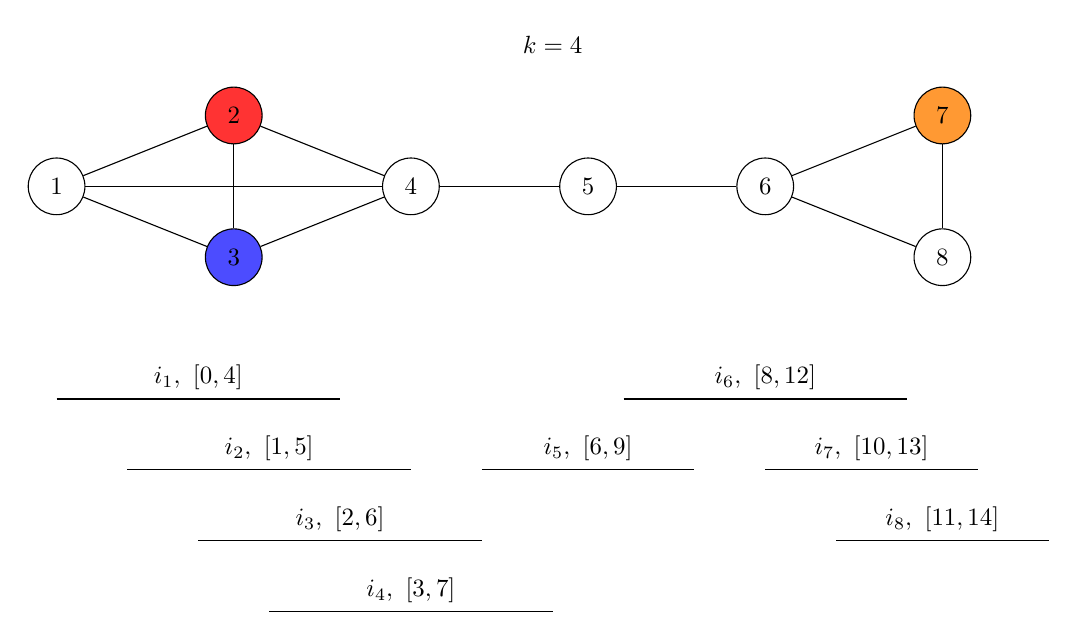
\begin{tikzpicture}[n/.style={circle,draw=black,minimum width=8mm}, scale=0.9, every
            node/.style={transform shape}]
            \node[n] (1) at (0,1) {$1$};
            \node[n,fill=red!80] (2) at (2.5,2) {$2$};
            \node[n,fill=blue!70] (3) at (2.5,0) {$3$};
            \node[n] (4) at (5,1) {$4$};
            \node[n] (5) at (7.5,1) {$5$};
            \node[n] (6) at (10,1) {$6$};
            \node[n,fill=orange!80] (7) at (12.5,2) {$7$};
            \node[n] (8) at (12.5,0) {$8$};

            \node (lab) at (7,3) {$k = 4$};

            \draw[-] (1) to (2);
            \draw[-] (1) to (3);
            \draw[-] (1) to (4);

            \draw[-] (2) to (3);
            \draw[-] (2) to (4);

            \draw[-] (3) to (4);

            \draw[-] (4) to (5);

            \draw[-] (5) to (6);

            \draw[-] (6) to (7);
            \draw[-] (6) to (8);
            
            \draw[-] (7) to (8);

            \draw[-] (0, -2) to node[above] {$i_1,\ [0,4]$} (4, -2);
            \draw[-] (1, -3) to node[above] {$i_2,\ [1,5]$} (5, -3);
            \draw[-] (2, -4) to node[above] {$i_3,\ [2,6]$} (6, -4);
            \draw[-] (3, -5) to node[above] {$i_4,\ [3,7]$} (7, -5);
            \draw[-] (6, -3) to node[above] {$i_5,\ [6,9]$} (9, -3);
            \draw[-] (8, -2) to node[above] {$i_6,\ [8,12]$} (12, -2);
            \draw[-] (10, -3) to node[above] {$i_7,\ [10, 13]$} (13, -3);
            \draw[-] (11, -4) to node[above] {$i_8,\ [11, 14]$} (14, -4);
        \end{tikzpicture}
    \end{center}
    \caption{Une instance de \precolor sur un graphe d'intervalles propre}
    \label{instance_precolor}
\end{figure}
% }}}

% {{{ FIGURES : Transformation
\begin{figure}
    \begin{center}
        % {{{ Precoloration
        \begin{minipage}[c][5cm][c]{0.35\linewidth}
            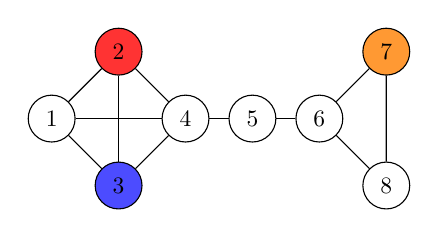
\begin{tikzpicture}[n/.style={circle,draw=black,minimum width=7mm},scale=0.85,every node/.style={transform shape}]
                \node[n] (1) at (0,1) {$1$};
                \node[n,fill=red!80] (2) at (1,2) {$2$};
                \node[n,fill=blue!70] (3) at (1,0) {$3$};
                \node[n] (4) at (2,1) {$4$};
                \node[n] (5) at (3,1) {$5$};
                \node[n] (6) at (4,1) {$6$};
                \node[n,fill=orange!80] (7) at (5,2) {$7$};
                \node[n] (8) at (5,0) {$8$};

                \draw[-] (1) to (2);
                \draw[-] (1) to (3);
                \draw[-] (1) to (4);

                \draw[-] (2) to (3);
                \draw[-] (2) to (4);

                \draw[-] (3) to (4);

                \draw[-] (4) to (5);

                \draw[-] (5) to (6);

                \draw[-] (6) to (7);
                \draw[-] (6) to (8);
                
                \draw[-] (7) to (8);
            \end{tikzpicture}
        \end{minipage}
        % }}}
        \hfill
        % {{{ Réservations
        \begin{minipage}[c][5cm][c]{0.55\linewidth}
            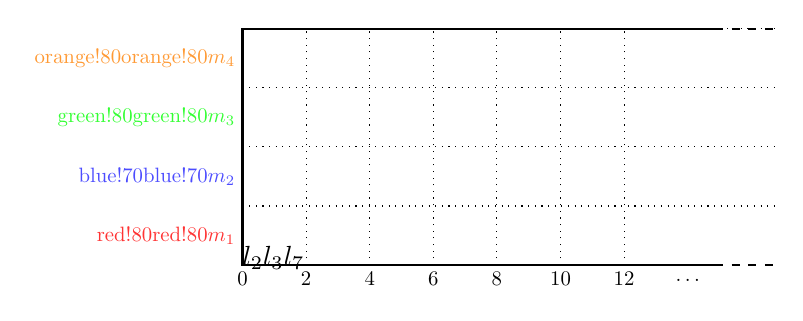
\begin{tikzpicture}[>=latex,scale=0.75,every node/.style={transform shape}]
                \pgfmathparse{2/13 * 7} \let\xpas\pgfmathresult
                \pgfmathparse{int(13/2)} \let\nbpas\pgfmathresult
                \pgfmathparse{\xpas/2} \let\unitxpas\pgfmathresult
                
                \draw[thick] (8,0) -- (0,0) -- (0,4) -- (8,4);
                \draw[thick,dashed] (8,0) -- (9,0);
                \draw[thick,dashed] (8,4) -- (9,4);

                \node[below] at (0, 0) {$0$};

                \foreach \x in {1,...,\nbpas}{
                    \pgfmathparse{\x * \xpas} \let\abscisse\pgfmathresult
                    \pgfmathparse{int(\x * 2)} \let\xlabel\pgfmathresult

                    \node[below] at (\abscisse, 0) {$\xlabel$};
                    \draw[dotted] (\abscisse,0) to (\abscisse,4);
                }

                \pgfmathparse{(\nbpas + 1) * \xpas} \let\abscisse\pgfmathresult
                \node[above] at (\abscisse, -0.4) {$\dots$};

                \foreach \y/\color in {1/red!80,2/blue!70,3/green!80,4/orange!80}{
                    \pgfmathparse{\y - 0.5} \let\ordlabel\pgfmathresult

                    \node[left, \color] at (0, \ordlabel) {$m_\y$};
                    \draw[dotted] (0, \y) to (9, \y);
                }

                \newlabeledresa{4}{1}{1}{$l_2$}
                \newlabeledresa{4}{2}{2}{$l_3$}
                \newlabeledresa{2}{4}{10}{$l_7$}
            \end{tikzpicture}
        \end{minipage}
        % }}}

        % {{{ Coloration
        \begin{minipage}[c][5cm][c]{0.35\linewidth}
            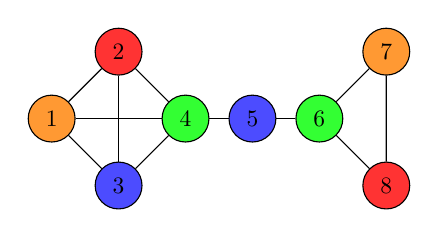
\begin{tikzpicture}[n/.style={circle,draw=black,minimum width=7mm},scale=0.85,every node/.style={transform shape}]
                \node[n,fill=orange!80] (1) at (0,1) {$1$};
                \node[n,fill=red!80] (2) at (1,2) {$2$};
                \node[n,fill=blue!70] (3) at (1,0) {$3$};
                \node[n,fill=green!80] (4) at (2,1) {$4$};
                \node[n,fill=blue!70] (5) at (3,1) {$5$};
                \node[n,fill=green!80] (6) at (4,1) {$6$};
                \node[n,fill=orange!80] (7) at (5,2) {$7$};
                \node[n,fill=red!80] (8) at (5,0) {$8$};

                \draw[-] (1) to (2);
                \draw[-] (1) to (3);
                \draw[-] (1) to (4);

                \draw[-] (2) to (3);
                \draw[-] (2) to (4);

                \draw[-] (3) to (4);

                \draw[-] (4) to (5);

                \draw[-] (5) to (6);

                \draw[-] (6) to (7);
                \draw[-] (6) to (8);
                
                \draw[-] (7) to (8);
            \end{tikzpicture}
        \end{minipage}
        % }}}
        \hfill
        % {{{ Ordonnancement
        \begin{minipage}[c][5cm][c]{0.55\linewidth}
            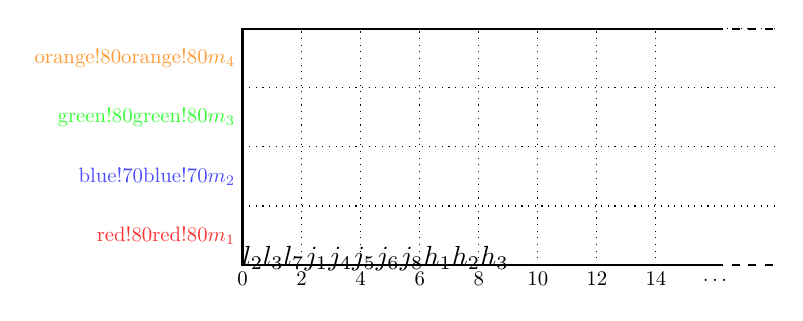
\begin{tikzpicture}[>=latex,scale=0.75,every node/.style={transform shape}]
                \pgfmathparse{2/14 * 7} \let\xpas\pgfmathresult
                \pgfmathparse{int(14/2)} \let\nbpas\pgfmathresult
                \pgfmathparse{\xpas/2} \let\unitxpas\pgfmathresult
                
                \draw[thick] (8,0) -- (0,0) -- (0,4) -- (8,4);
                \draw[thick,dashed] (8,0) -- (9,0);
                \draw[thick,dashed] (8,4) -- (9,4);

                \node[below] at (0, 0) {$0$};

                \foreach \x in {1,...,\nbpas}{
                    \pgfmathparse{\x * \xpas} \let\abscisse\pgfmathresult
                    \pgfmathparse{int(\x * 2)} \let\xlabel\pgfmathresult

                    \node[below] at (\abscisse, 0) {$\xlabel$};
                    \draw[dotted] (\abscisse,0) to (\abscisse,4);
                }

                \pgfmathparse{(\nbpas + 1) * \xpas} \let\abscisse\pgfmathresult
                \node[above] at (\abscisse, -0.4) {$\dots$};

                \foreach \y/\color in {1/red!80,2/blue!70,3/green!80,4/orange!80}{
                    \pgfmathparse{\y - 0.5} \let\ordlabel\pgfmathresult

                    \node[left, \color] at (0, \ordlabel) {$m_\y$};
                    \draw[dotted] (0, \y) to (9, \y);
                }

                \newlabeledresa{4}{1}{1}{$l_2$}
                \newlabeledresa{4}{2}{2}{$l_3$}
                \newlabeledresa{2}{4}{10}{$l_7$}

                \newtask{4}{4}{0}{$j_1$}
                \newtask{4}{3}{3}{$j_4$}
                \newtask{3}{2}{6}{$j_5$}
                \newtask{4}{3}{8}{$j_6$}
                \newtask{3}{1}{11}{$j_8$}

                \newhole{6}{1}{5}{$h_1$}
                \newhole{1}{3}{7}{$h_2$}
                \newhole{6}{4}{4}{$h_3$}
            \end{tikzpicture}
        \end{minipage}
        % }}}
    \end{center}
    \caption{Illustration du principe de la transformation polynomiale}
    \label{fig_transpoly}
\end{figure}
% }}}
\end{ex}
% }}}

% }}}

\appendix
\bibliographystyle{plain}
\bibliography{biblio}


\end{document}
